%
% File: chap02.tex
%
\let\textcircled=\pgftextcircled
\chapter{Experimental Results}
\label{Chapter4}
The number of partitions was set to three 

For the dataset used to train and test the algorithm "The Graph Partitioning Archive"~\cite{archive}
The graphs are in the standard format used by JOSTLE and METIS. A description of the format and the requirements can be found in~\cite{jostle}.

For the purposes of this research, the graphs contained in "The Graph Partitioning Archive" where categorized in one of the following categories according to their vertex cardinality: 
\begin{itemize}
    \item Tiny graphs: those with less than $10,000$ nodes,
    \item Small graphs: those with node size between $45,000$ and $75,000$ and,
    \item Medium graphs: those with at least $99,000$ nodes but no more than $500,000$.
\end{itemize}

Ask Luis: is there a word for graphs with size more than big

\begin{table}
\centering
\begin{tabular}{ |p{1.75cm}||cc|  }
\hline
\multicolumn{3}{|c|}{\textbf{Computation Graphs}} \\
\hline
\hline
\textbf{Name} & \textbf{Nodes} & \textbf{Edges} \\
\hline
data & 2851 & 15093  \\
add32 & 4960 & 9462  \\
bcsstk33 & 8738 & 291583  \\
crack & 10240 & 30380  \\
\hline
fe\_body & 45087 & 163734  \\
t60k & 60005 & 89440  \\
wing & 62032 & 121544  \\
finan512 & 74752 & 261120 \\
\hline
fe\_rotor & 99617 & 662431  \\
598a & 110971 & 741934  \\
m14b & 214765 & 1679018	 \\
auto & 448695 & 3314611  \\
\hline
\end{tabular}
\caption{\label{tab:results}Summary of the graphs characteristics. Taken from "The Graph Partitioning Archive" ~\cite{archive}}
\end{table}

In table 

\begin{table}
\centering
\begin{tabular}{ |p{1.75cm}||cc|cc|cc|  }
%\hline
%\multicolumn{3}{|c|}{\textbf{Results}} \\
\hline
\hline
\textbf{Graphs} & \multicolumn{2}{c}{\textbf{METIS}} & \multicolumn{2}{c}{\textbf{GAP}} & \multicolumn{2}{c|}{\textbf{Modified GAP}} \\
\hline
\hline
Name & Edge Cut & Balancedness & Edge Cut & Balancedness & Edge Cut & Balancedness \\
\hline
data & 0 & 0 & 0 & 0 & 0 & 0  \\
add32 & 0 & 0 & 0 & 0 & 0 & 0  \\
bcsstk33 & 0 & 0 & 0 & 0 & 0 & 0  \\
crack & 0 & 0 & 0 & 0 & 0 & 0  \\
\hline
fe\_body & 0 & 0 & 0 & 0 & 0 & 0  \\
t60k & 0 & 0 & 0 & 0 & 0 & 0  \\
wing & 0 & 0 & 0 & 0 & 0 & 0  \\
finan512 & 0 & 0 & 0 & 0 & 0 & 0  \\
\hline
fe\_rotor & 0 & 0 & 0 & 0 & 0 & 0  \\
598a & 0 & 0 & 0 & 0 & 0 & 0  \\
m14b & 0 & 0 & 0 & 0 & 0 & 0  \\
auto & 0 & 0 & 0 & 0 & 0 & 0  \\
\hline
\end{tabular}
\caption{\label{tab:comp_graphs}Comparison of the results obtained by different algorithms in the computation graphs}
\end{table}

%%%%%%%%%%%%%%%%%%%%%%%%%%%%%%%%%%%%%%%%%%%%%% Small graph histograms %%%%%%%%%%%%%%%%%%%%%%%%%%%%%%%%%%%%%%%%%%%%%%

\begin{figure}[h!]
\centering
\begin{subfigure}[b]{.35\textwidth}
  \centering
  % include first image
  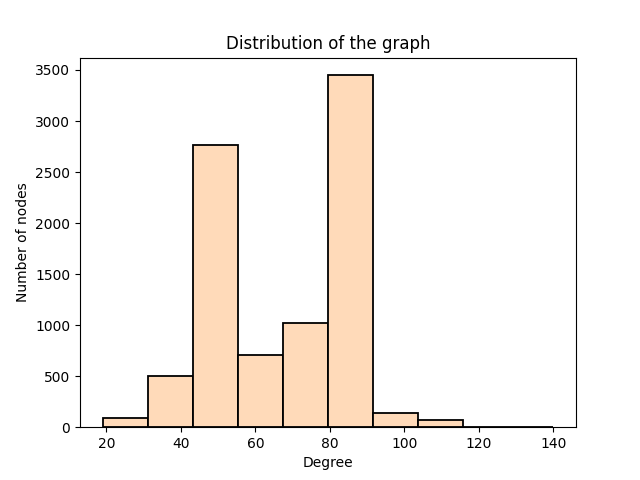
\includegraphics[width=\linewidth]{small_graphs/bcsstk33.png}  
  \caption{bcsstk33}
  \label{fig:sub-first}
\end{subfigure}
\begin{subfigure}[b]{.35\textwidth}
  \centering
  % include second image
  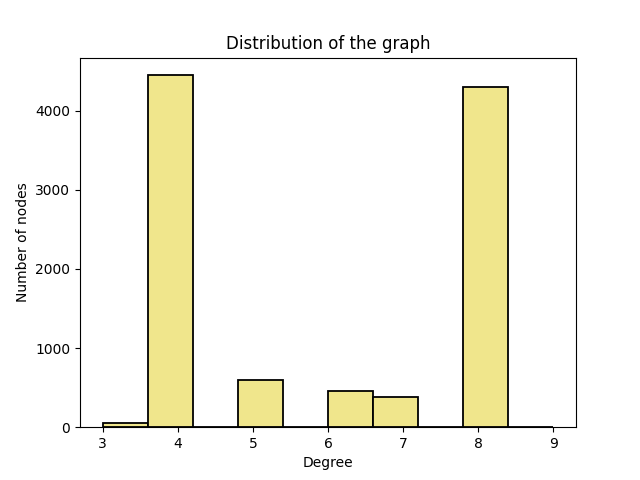
\includegraphics[width=\linewidth]{small_graphs/crack.png}  
  \caption{crack}
  \label{fig:sub-second}
\end{subfigure}

\begin{subfigure}[b]{.35\textwidth}
  \centering
  % include third image
  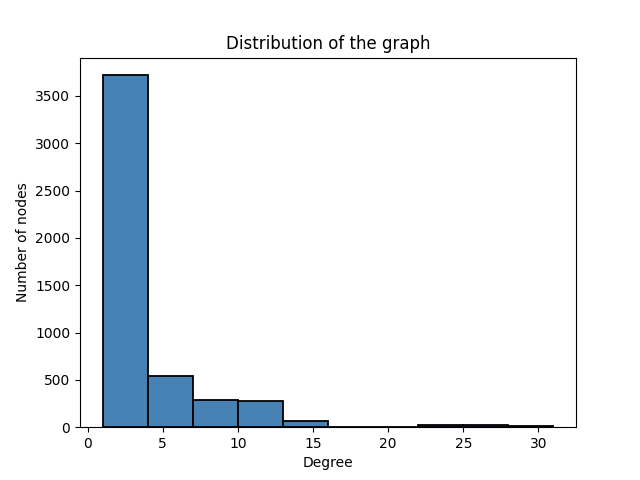
\includegraphics[width=\linewidth]{small_graphs/add32.png}  
  \caption{add32}
  \label{fig:sub-third}
\end{subfigure}
\begin{subfigure}[b]{.35\textwidth}
  \centering
  % include fourth image
  \includegraphics[width=\linewidth]{small_graphs/data.png}  
  \caption{data}
  \label{fig:sub-fourth}
\end{subfigure}
\caption{Degree histogram of small graphs: bcsstk33, crack, add32, and data. Graphs are not so dense.}
\label{fig:fig}
\end{figure}

%%%%%%%%%%%%%%%%%%%%%%%%%%%%%%%%%%%%%%%%%% Medium graph histograms %%%%%%%%%%%%%%%%%%%%%%%%%%%%%%%%%%%%%%%%%%%%%%

\begin{figure}[h!]
\centering
\begin{subfigure}{.35\textwidth}
  \centering
  % include first image
  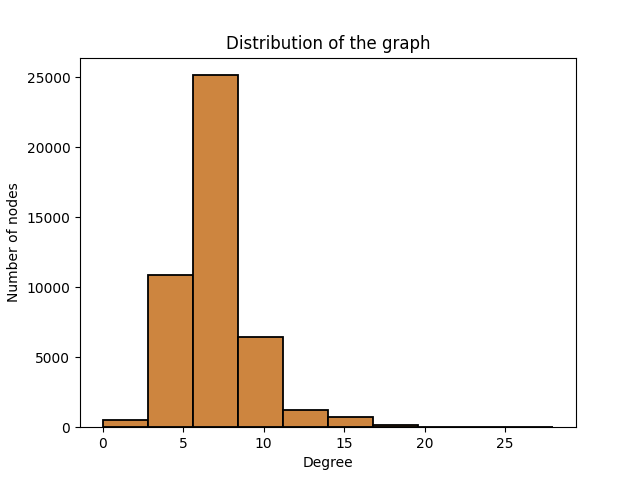
\includegraphics[width=\linewidth]{medium_graphs/fe_body.png}  
  \caption{fe\_body}
  \label{fig:sub-first}
\end{subfigure}
\begin{subfigure}{.35\textwidth}
  \centering
  % include second image
  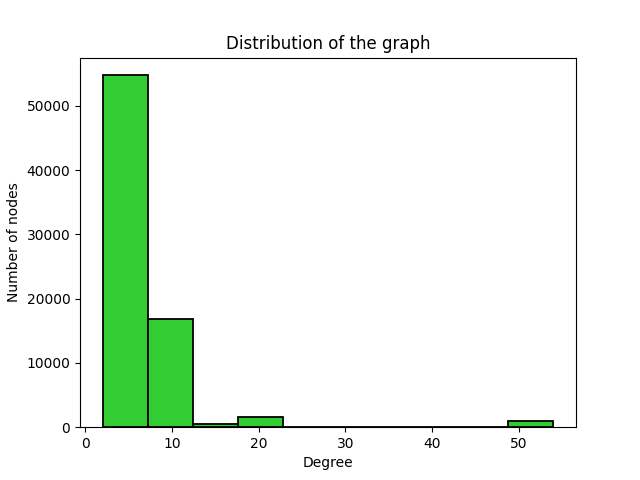
\includegraphics[width=\linewidth]{medium_graphs/finan512.png}  
  \caption{finan512}
  \label{fig:sub-second}
\end{subfigure}

\begin{subfigure}{.35\textwidth}
  \centering
  % include third image
  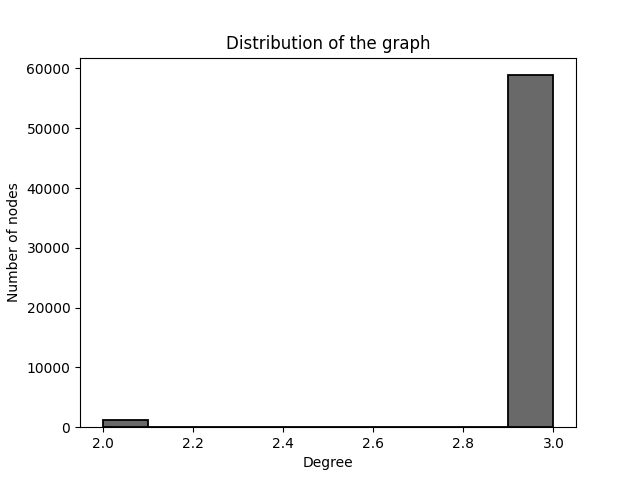
\includegraphics[width=\linewidth]{medium_graphs/t60k.png}  
  \caption{t60k}
  \label{fig:sub-third}
\end{subfigure}
\begin{subfigure}{.35\textwidth}
  \centering
  % include fourth image
  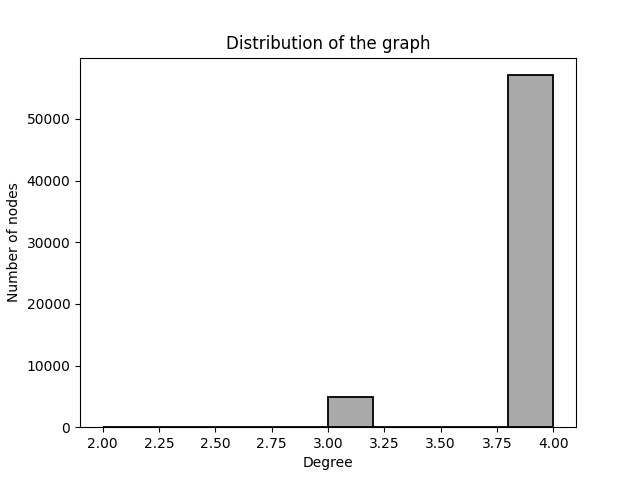
\includegraphics[width=\linewidth]{medium_graphs/wing.png}  
  \caption{wing}
  \label{fig:sub-fourth}
\end{subfigure}
\caption{Degree histogram of medium graphs. Graphs are not so dense.}
\label{fig:fig}
\end{figure}

%%%%%%%%%%%%%%%%%%%%%%%%%%%%%%%%%%%%%%%%%%%%%% Large graph histograms %%%%%%%%%%%%%%%%%%%%%%%%%%%%%%%%%%%%%%%%%%%%%%

\begin{figure}[h!]
\centering
\begin{subfigure}{.35\textwidth}
  \centering
  % include first image
  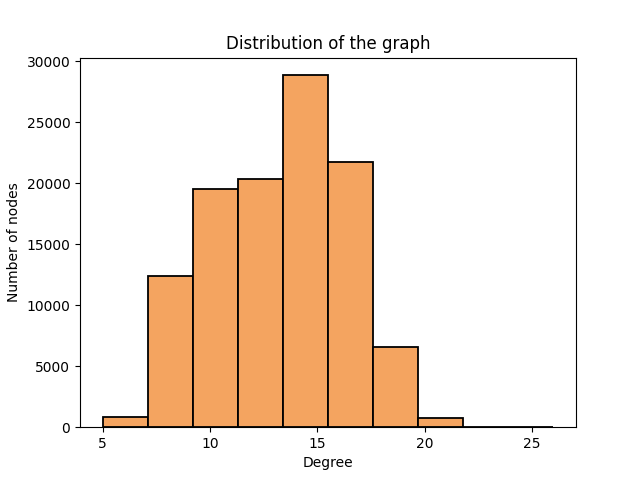
\includegraphics[width=\linewidth]{large_graphs/598a.png}  
  \caption{598a}
  \label{fig:sub-first}
\end{subfigure}
\begin{subfigure}{.35\textwidth}
  \centering
  % include second image
  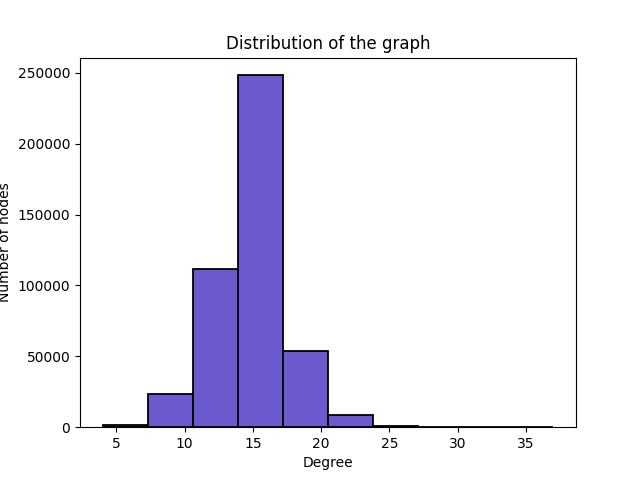
\includegraphics[width=\linewidth]{large_graphs/auto.png}  
  \caption{auto}
  \label{fig:sub-second}
\end{subfigure}

\begin{subfigure}{.35\textwidth}
  \centering
  % include third image
  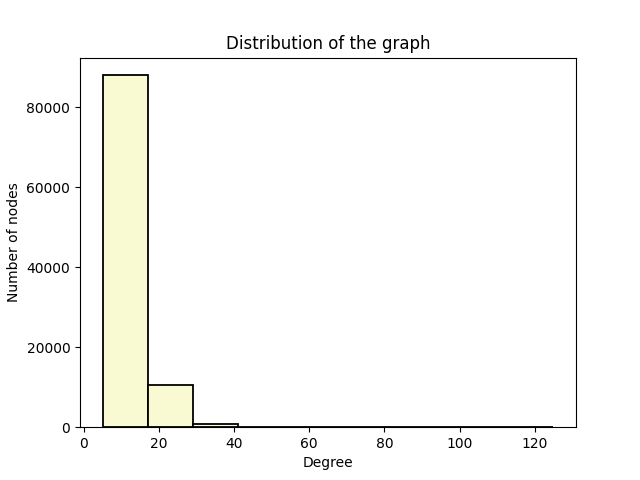
\includegraphics[width=\linewidth]{large_graphs/fe_rotor.png}  
  \caption{fe\_rotor}
  \label{fig:sub-third}
\end{subfigure}
\begin{subfigure}{.35\textwidth}
  \centering
  % include fourth image
  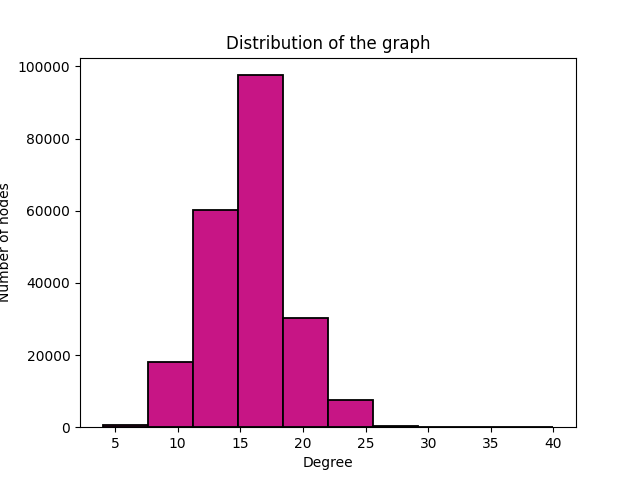
\includegraphics[width=\linewidth]{large_graphs/m14b.png}  
  \caption{m14b}
  \label{fig:sub-fourth}
\end{subfigure}
\caption{Degree histogram of large graphs. Graphs are not so dense.}
\label{fig:fig}
\end{figure}

%%%%%%%%%%%%%%%%%%%%%%%%%%%%%%%%%%%%%%%%%%%%%% Graph images %%%%%%%%%%%%%%%%%%%%%%%%%%%%%%%%%%%%%%%%%%%%%%%%%%%
\begin{comment}
\begin{figure}[h!]
\centering
\begin{subfigure}{.35\textwidth}
  \centering
  % include first image
  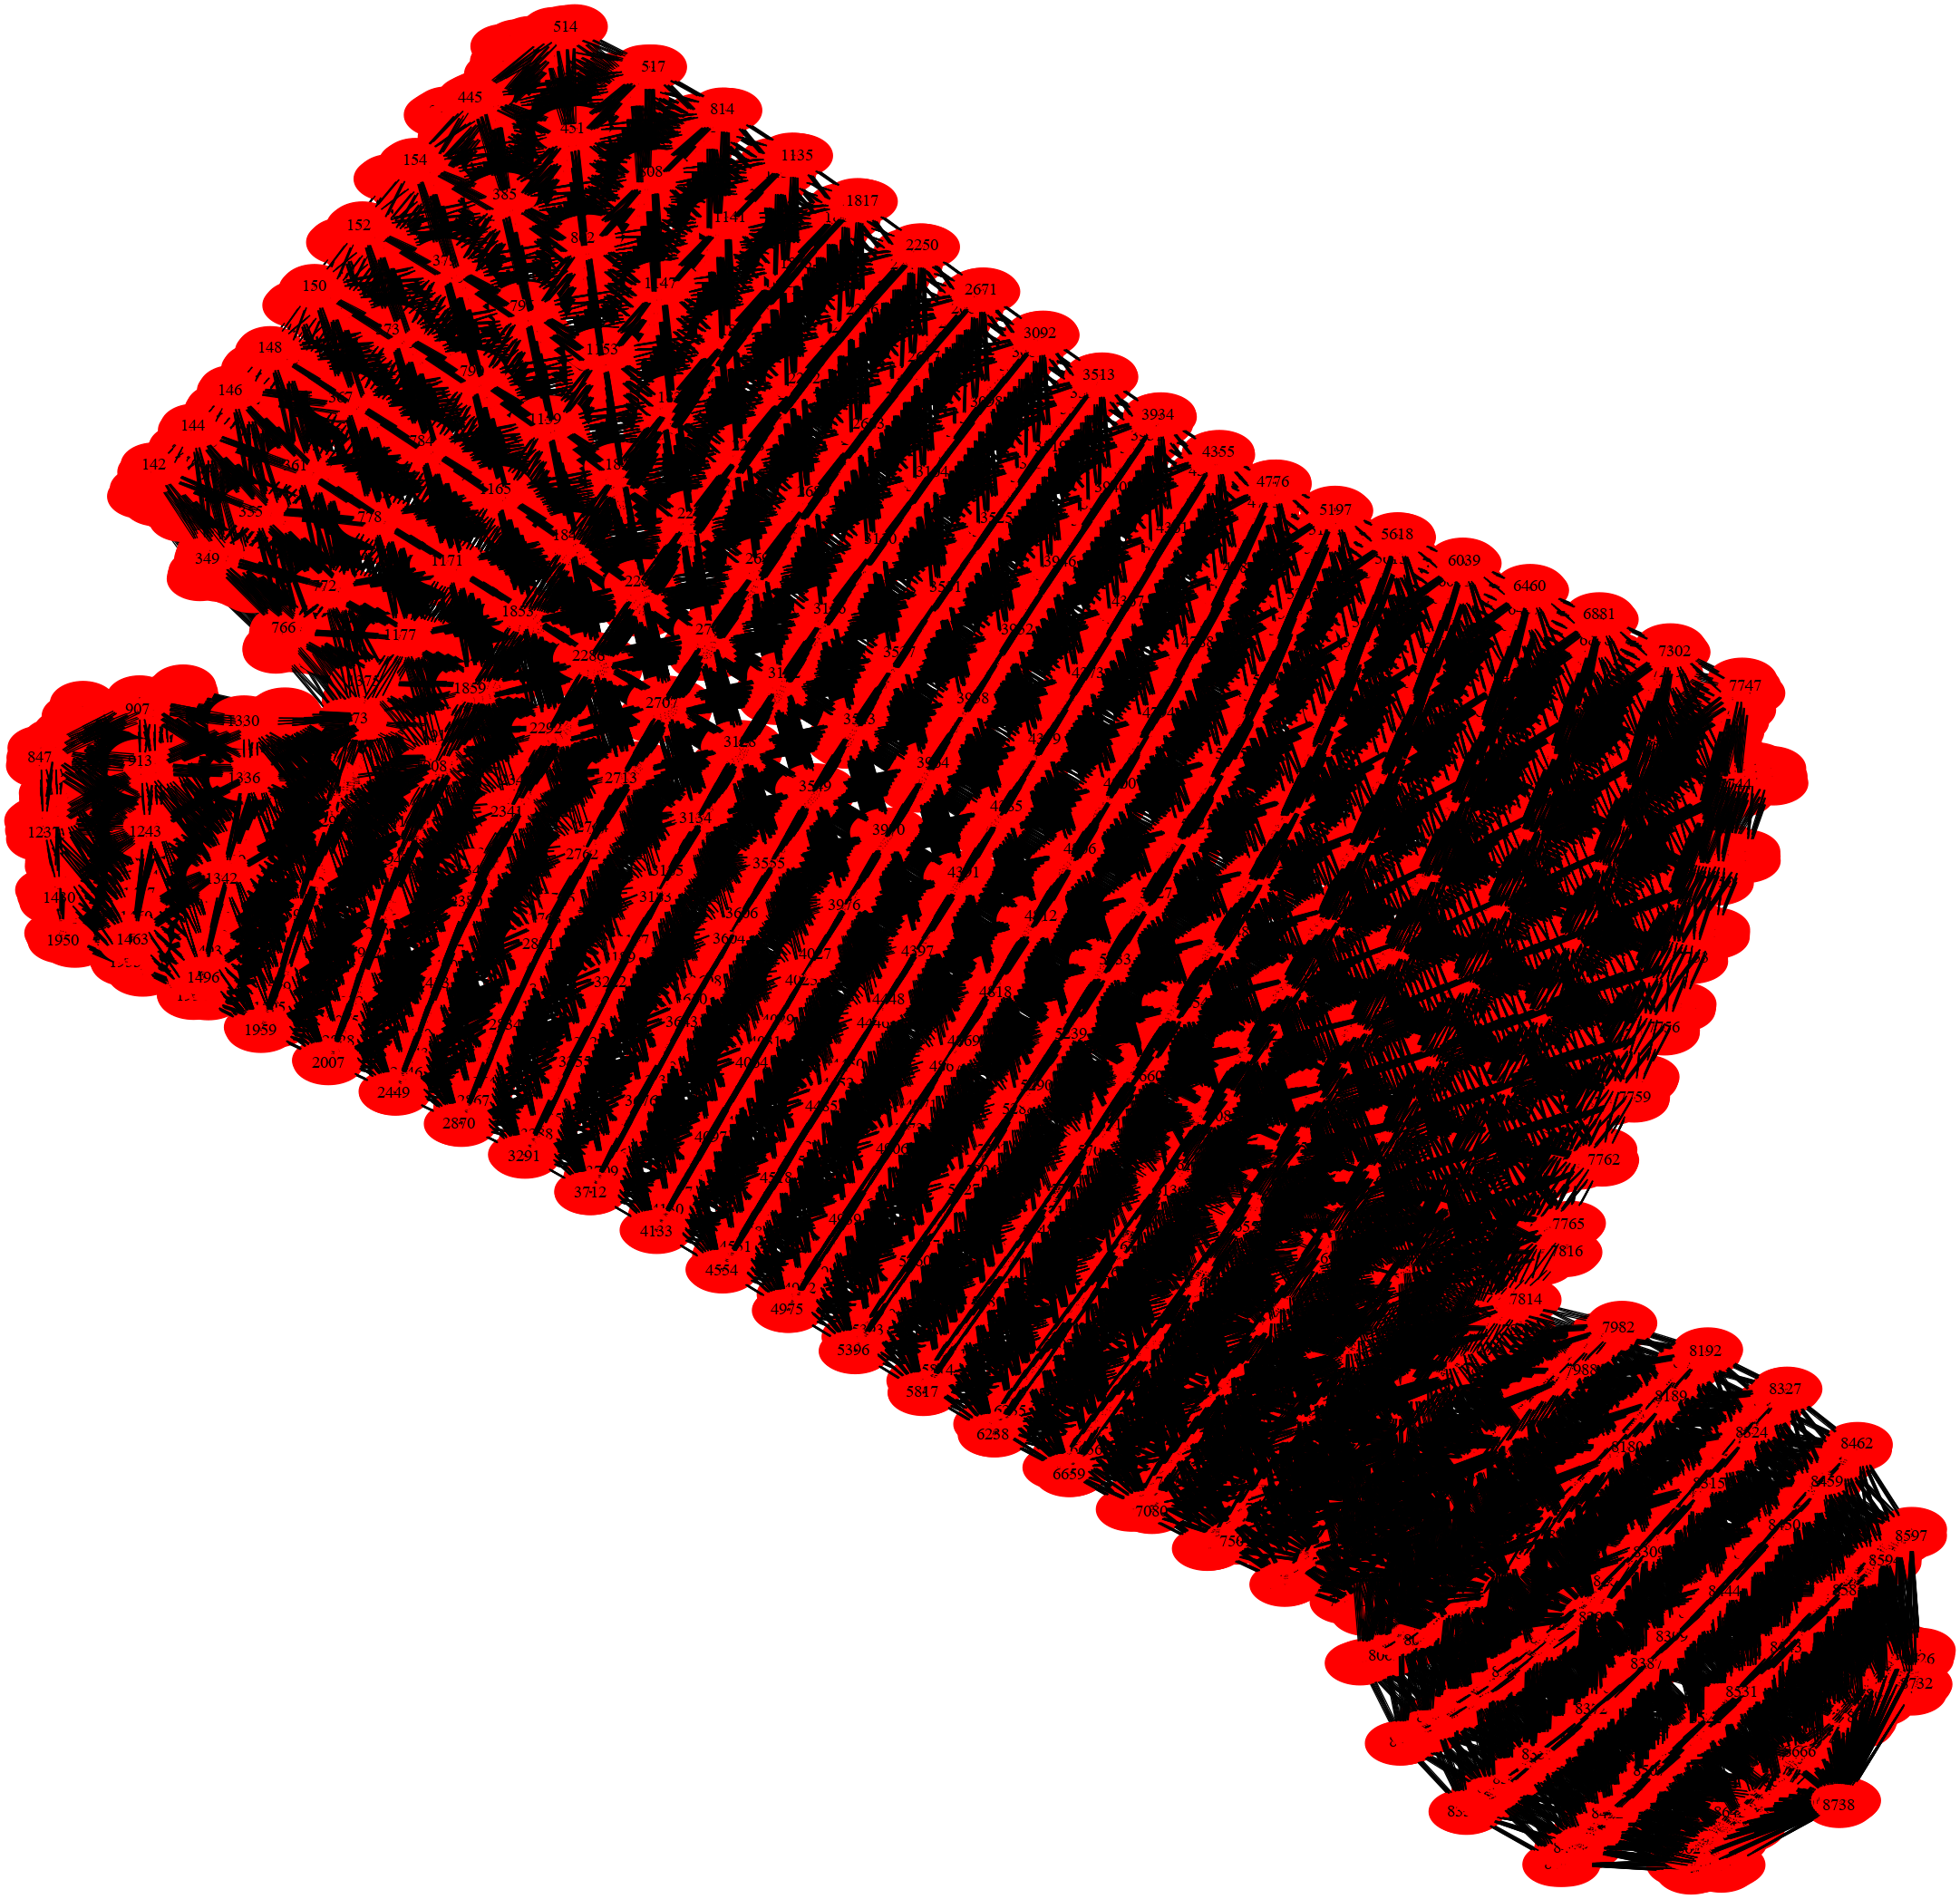
\includegraphics[width=0.7\linewidth]{graphs/bcsstk33.png}  
  \caption{bcsstk33}
  \label{fig:sub-first}
\end{subfigure}
\begin{subfigure}{.35\textwidth}
  \centering
  % include second image
  \includegraphics[width=0.7\linewidth]{graphs/crack-min.png}  
  \caption{crack}
  \label{fig:sub-second}
\end{subfigure}

\begin{subfigure}{.35\textwidth}
  \centering
  % include third image
  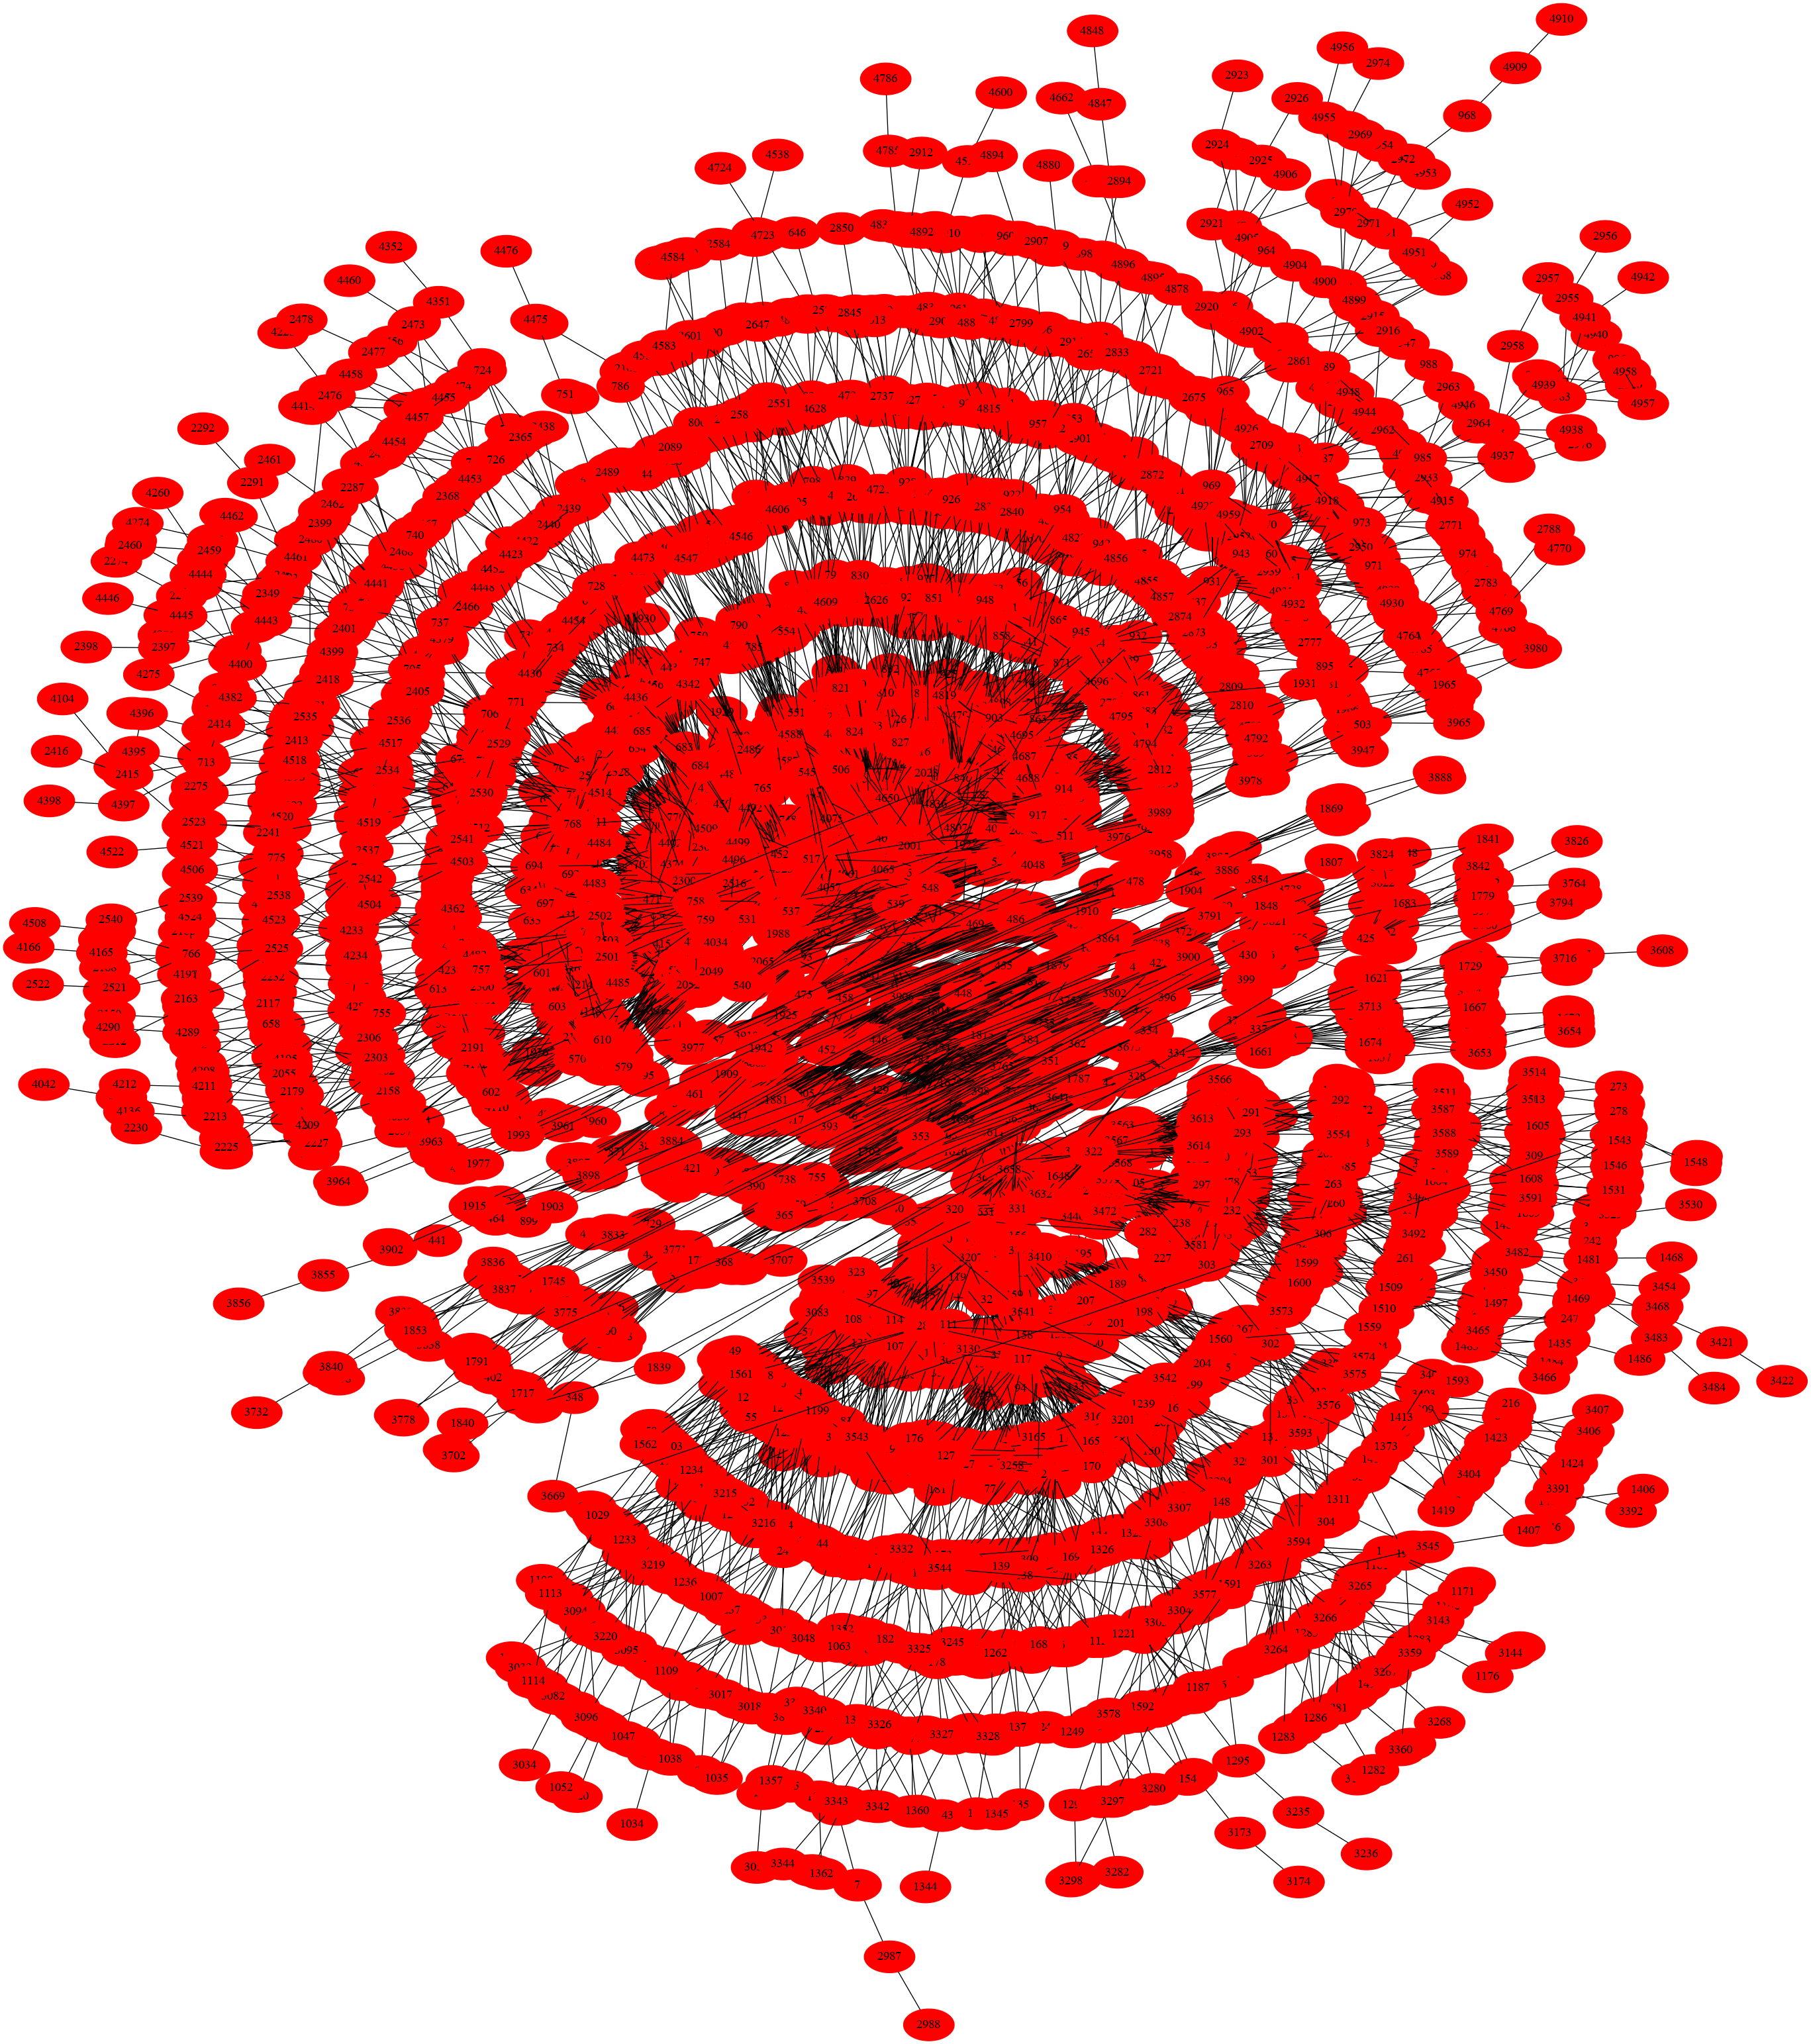
\includegraphics[width=0.7\linewidth]{graphs/add32.png}  
  \caption{add32}
  \label{fig:sub-third}
\end{subfigure}
\begin{subfigure}{.35\textwidth}
  \centering
  % include fourth image
  \includegraphics[width=0.7\linewidth]{graphs/data.png}  
  \caption{data}
  \label{fig:sub-fourth}
\end{subfigure}
\caption{Visualization of some of the graphs used in the experiments.}
\label{fig:fig}
\end{figure}
\end{comment}